%Template pembuatan proposal skripsi.
\documentclass{jtetiproposalskripsi}

%-----------------------------------------------------------------
%Disini awal masukan untuk data proposal skripsi
%-----------------------------------------------------------------
\titleind{PERANCANGAN JARINGAN HOTSPOT SERVER BERBASIS MIKROTIK DI GEDUNG SEKOLAH DASAR}

\fullname{HENDRO SUSANTO}

\idnum{1210652053}

\approvaldate{13 Januari 2015}

\degree{Sarjana Komputer}

\yearsubmit{2015}

\program{Teknik Informatika}

\headprogram{Sarjiya, S.T., M.T., Ph.D.}

\dept{Teknologi Informatika}

\firstsupervisor{Triawan Adi Cahyanto}




%-----------------------------------------------------------------
%Disini akhir masukan untuk data proposal skripsi
%-----------------------------------------------------------------

\begin{document}

\cover

\approvalpage

%-----------------------------------------------------------------
%Disini akhir masukan untuk muka skripsi
%-----------------------------------------------------------------

%-----------------------------------------------------------------
%Disini awal masukan Intisari
%-----------------------------------------------------------------
\begin{abstractind}
Komunikasi tanpa kabel/nirkabel (\emph{Wireless}) telah menjadi kebutuhan dasar atau gaya hidup baru masyarakat informasi. LAN nirkabel yang lebih dikenal dengan jaringan Wi-Fi menjadi teknologi alternatif dan relatif lebih mudah untuk diimplementasikan di lingkungan kerja. Instalasi perangkat jaringan Wi-Fi lebih fleksibel karena tidak membutuhkan penghubung kabel antar komputet. \emph{Access point} merupakan perangkat yang biasa digunakan dalam jaringan \emph{wireless} (\emph{Hotspot area}) dimana user atau pengguna terhubung ke internet menggunakan media udara melalui perangkat \emph{access point}. Selain itu, dengan jaringan berbasis wireless ini membuat masyarakat lebih mudah untuk mengakses internet dimanapun berada. Implementasi pemasangan jaringan ini terdiri dari pemasangan konektor RJ- 45 pada kabel UTP, melakukan konfigurasi \emph{repeater}, konfigurasi \emph{Access Point}, konfigurasi \emph{HotSpot Server MikroTik}. Dengan adanya jaringan wireless berbasis \emph{HotSpot} di Sekolah Dasar, akan mempermudah siswa/i untuk mengakses internet dengan gratis. Selain itu, melakukan konfigurasi jaringan wireless tidak begitu sulit, asalkan mengikuti aturan pembuatan jaringan.
\bigskip

Kata Kunci : \emph{Wireless}, Tugas akhir,\emph{MikroTik}, \emph{HotSpot}, dan \emph{Access Point}.

\end{abstractind}
%-----------------------------------------------------------------
%Disini akhir masukan Intisari
%-----------------------------------------------------------------

\tableofcontents
\addcontentsline{toc}{chapter}{DAFTAR ISI}
\selectlanguage{bahasa}\clearpage\pagenumbering{arabic}\setcounter{page}{1}

%-----------------------------------------------------------------
%Disini awal masukan untuk Bab
%-----------------------------------------------------------------
\chapter{LATAR BELAKANG}

\section{Latar Belakang Masalah}
Sekolah adalah sebuah lembaga yang dirancang untuk pengajaran siswa (atau "murid") dibawah pengawasan Guru. Sebagian besar negara memiliki sistem pendidikan formal, yang umumnya wajib. Dalam sistem ini, siswa kemajuan melalui serangkaian sekolah. Nama-nama untuk sekolah-sekolah ini bervariasi menurut negara, tetapi umumnya termauk sekolah dasar untuk anak-anak muda dan sekolah menengah untuk remaja yang telah menyelesaikan pendidikan dasar.

Selain sekolah-sekolah inti, siswa di negara tertentu juga mungkin memiliki akses dan mengikuti sekolah-sekolah baik sebelum dan sesudah pendidikan dasar dan menengah. TK atau pra-sekolah menyediakan sekolah beberapa anak-anak yang sangat muda (biasanya umur 3-5 tahun). Universitas, sekolah kejuruan, perguruan tinggi atau seminari mungkin tersedia setelah sekolah menengah. Sebuah sekolah mungkin juga didedikasikan untuk satu bidang tertentu, seperti sekolah ekonomi atau tari. Alternatif sekolah dapat
menyediakan kurikulum dan metode non-tradisional.

Ada juga sekolah non-pemerintah, yang disebut sekolah swasta mungkin untuk anak-anak dengan kebutuhan khusus ketika pemerintah tidak bisa memberi sekolah khusus bagi mereka; keagamaan, seperti sekolah Islam, sekolah Kristen, hawzas, yeshivas dab lain-lain, atau sekolah yang memiliki standar pendidikan yang lebih tinggi atau berusaha untuk mengembangkan prestasi pribadi lainnya. Sekolah untuk orang dewasa meliputi lembaga-lembaga pelatihan perusahaan dan pendidikan dan pelatihan militer. Dalam \emph{homeschooling} dan sekolah \emph{online}, pengajaran berlangsung di luar gedung sekolah tradisional.

Dimana untuk meningkatkan proses belajar mengajar saat ini di lingkungan sekolah tidak hanya sumber materi dari buku catatan. Guru-guru bisa mengakses materi pelajaran dari internet untuk menunjang proses belajar mengajarnya. Dengan luas sekolah yang cukup besar, terdiri dari ruang-ruang kelas yang dipenuhi oleh siswa-siswi, internet sudah menjadi salh satu kebutuhan pokok setiap hari untuk proses belajar mengajar. Maka dari itu disediakanlah fasilitas HotSpot bagi siswa dan gueu untuk mengakses internet.

Dewasa ini banyak system routing yang digunakan, daro yang gratis (free) sampai yang nernayar, dari mudah sampai yang sudah dalam sistem konfigurasinya. Salah satunya yang akan kita bahas adalah Mikrotik RouterOS, yaitu sistem operasi router yang sekarang ini banyak di gunakan oleh warnet-warnet, kantor-kantor ataupun instansi-instansi lain. Minkrotik RouterOS merupakan router network yang handal, dilengkapi dengan berbagai fitur dan tools, baik untuk jaringan kabel maupun jaringan tanpa kabel (wireless). Salah satu fitur yang disediakan oleh Mikrotik yang akan dibahas adalah Hotspot Server.

\section{Rumusan Masalah}
Berdasarkan latar belakang diatas dapat dirumuskan suatu permasalahan pada sekolah-sekolah yaitu :
\begin{enumerate}
\item Bagaimana membangun sebuah jaringan wireless berbasis Hotspot dengan menggunakan Mikrotik sebagai server.
\item Bagaimana mengatasi lemahnya sinyal wireless dengan menambah repeater sebagai penguat sinyal.
\end{enumerate}

\section{Batasan Masalah}
Adapun batasan masalah dalam perancangan jaringan hotpsot server ini yaitu:
\begin{enumerate}
\item Membahas perancangan Hotspot server berbasis Mikrotik menggunakan jaringan wireless sebagai media jaringan Hotspot.
\item Ruang lingkup masalah ini membahas tentang rancangan sistem jaringan menggunakan jaringan wireless dengan WDS (Wireless Distribution System).
\end{enumerate}

\section{Tujuan Penelitian}
Adapun batasan masalah dalam perancangan jaringan hotpsot server ini yaitu:
\begin{enumerate}
\item Membahas perancangan Hotspot server berbasis Mikrotik menggunakan jaringan wireless sebagai media jaringan Hotspot.
\item Ruang lingkup masalah ini membahas tentang rancangan sistem jaringan menggunakan jaringan wireless dengan WDS (Wireless Distribution System).
\end{enumerate}

\section{Manfaat Penelitian}
Adapun manfaat dari pembuatan sistem hotspot ini adalah untuk mengetahui sedikit tidaknya tentang konsep jaringan serta konfigurasinya dan sedikit mengetahui kelebihan dan kekurangan menggunakan topologi WDS (Wrieless Distribution System).

%-------------------------------------------------------------------------------
\chapter{DASAR TEORI}                

\section{Jaringan}
Sebuah jaringan terdiri dari 2 atau lebih komputer yang saling berhubungan antara satu dengan yang lain, dan saling berbagi informasi. Konsep jringan komputer lahir pada tahun 1940-an di Amerika, dari group riset Harvard University yang dipimpin oleh profesor H. Aiken. Pada mulanya proyek tersebut hanyalah ingin memanfaatkan sebuah perangkat komputer yang harus dipakai bersama. Untuk mengerjakan beberapa proses tanpa banyak membuang waktu kosong maka dibuatlah proses beruntun (Batch Processing), sehingga beberapa program bisa di jalankan dalam sebuah komputer dengan kaidah antrian. Ada beberapa jenis jaringan, yaitu :

\begin{enumerate}
\item \emph{Local Area Network (LAN)}

\emph{LAN} adalah jaringan yang dibatasi oleh area yang relatif kecil, umumnya dibatasi oleh area lingkungan.
\item \emph{Metropolitan Area Network (MAN)}

\emph{MAN} biasanya meliputi area yang lebih besar dari \emph{LAN}, misalnya antar wilayah dalam satu propinsi yang menggabungkan jaringan \emph{LAN}.
\item \emph{Wide Area Network (WAN)}

\emph{WAN} adalah jaringan yang lingkupnya biasanya sudah menggunakan sarana satelit ataupun kabel bawah laut.
\end{enumerate}

\section{Wifi}
Wi-Fi juga ditulis Wifi atau WiFi adalah sebuah teknologi terkenal yang memanfaatkan peralatan elektronik untuk bertukar data secara nirkabel (menggunakan gelombang radio) melalui sebuah jaringan komputer, termasuk koneksi Internet berkecepatan tinggi. Wi-Fi Alliance mendefinisikan Wi-Fi sebagai "produk jaringan wilayah lokal nirkabel (WLAN) apapun yang didasarkan pada standar \emph{Institute of Electrical and Electronics Engineers} (IEEE) 802.11". Meski begitu, karena kebanyakan WLAN zaman sekarang didasarkan pada standar tersebut, istilah "Wi-Fi" dipakai dalam bahasa Inggris umum sebagai sinonim "WLAN".

\section{WDS \emph{(Wireless Distribution System)}}
\emph{Wireless Distribution System} (WDS) yang disebut juga sebagai \emph{Wireless Repeater} merupakan sistem untuk mengembangkan jaringan nirkabel tanpa harus menggunakan kabel sebagai \emph{backbone} untuk \emph{access point}, melainkan memanfaatkan jalur nirkabel dari access point. Kekurangan repeater adalah bisa mengurangi performansi wireless LAN. Repeater harus menerima dan mengirim setiap frame pada kanal radio yang sama, mengakibatkan terjadinya peggandaan jumlah trafic pada jaringan. Hal ini terjadi jika digunakan banyak repeater.

\section{MikroTik RouterOS}
MikroTik RouterOS adalah sistem operasi dan perangkat lunak yang dapat digunakan untuk menjadikan komputer manjadi router network yang handal, mencakup berbagai fitur yang dibuat untuk ip network dan jaringan wireless, cocok digunakan oleh ISP dan provider hotspot.

MikroTik adalah perusahaan kecil berkantor pusat di Latvia, yang dibentuk oleh John Trully dan Arnis Riekstins. Tahun 1996 John dan Arnis memulai dengan sistem Linux dan MS DOS yang dikombinasikan dengan teknologi Wireless LAN (W-LAN) Aeronet berkecepatan 2Mbps di Moldova. Barulah kemudian melayani lima pelanggannya di Latvia, karena ambisi mereka adalah membuat satu peranti lunak router yang handal dan disebarkan ke seluruh dunia. Prinsip dasar MikroTik bukan membuat Wireless ISP (WISP), tapi membuat program router yang handal dan dapat dijalankan di seluruh dunia. Hingga kini, MikroTik telah melayani sekitar empat ratusan pelanggannya.

Linux yang mereka gunakan pertama kali adalah Kernel 2.2 yang dikembangkan secara bersama-sama dengan bantuan 5 - 15 orang staf R dan D Mikrotik yang sekarang menguasai dunia routing di negara-negara berkembang. Selain staf di lingkungan Mikrotik, menurut Arnis, mereka merekrut juga tenagatenaga lepas dan pihak ketiga yang dengan intensif mengembangkan Mikrotik secara maraton.(http://id.wikipedia.org/wiki/MikroTik)


\section{HotSpot}
Hotspot (Wi-Fi) adalah salah satu bentuk pemanfaatan teknologi Wireless LAN pada lokasi-lokasi publik seperti taman, perpustakaan, restoran ataupun bandara. Pertama kali digagas tahun 1993 oleh Brett Steward. Hotspot juga dikenal dengan istilah captive portal. Cactive Portal akan menagkap semuatrafik dari klien dan akan memeriksa apakah klien tersebut sudah terotentikasi atau belum untuk menggunakan sumber daya jaringan. Jika belum maka klien tersebut akan diperiksa untuk melakukan otentikasi terlebih dahulu.(Imam Cartealy,2013). 

Salah satu fitur terkenal di dalam mikrotik yang merupakan salah satu metode untuk memberikan akses/layanan internet di area public dengan melalui proses autentikasi seperti yang sudah disebutkan sebelumnya, media yang digunakan bisa menggunakan kabel ataupun wireless. Cara kerja dari hotspot server ini dalam bentuk sederhana, hotspot akan melakukan block semua akses user dan user akan diminta untuk melakukan login via web browser. Apabila username dan password yang diisikan oleh user cocok dengan database hotspot, maka layanan akses akan diberikan. Kami akan memberikan contoh konfigurasi bagaimana cara mengintegrasikan 2 hotspot server yang sudah ada di 2 router yang berbeda (router A dan router B) dengan sebuah database UserManager yang akan terpasang di salah satu router (router A). (http://mikrotik.co.id) Topologinya bisa seperti yang ditunjukan pada Gambar 2.2 :

\vspace{-0.5cm}
\begin{figure}[ht!]
  \centering
    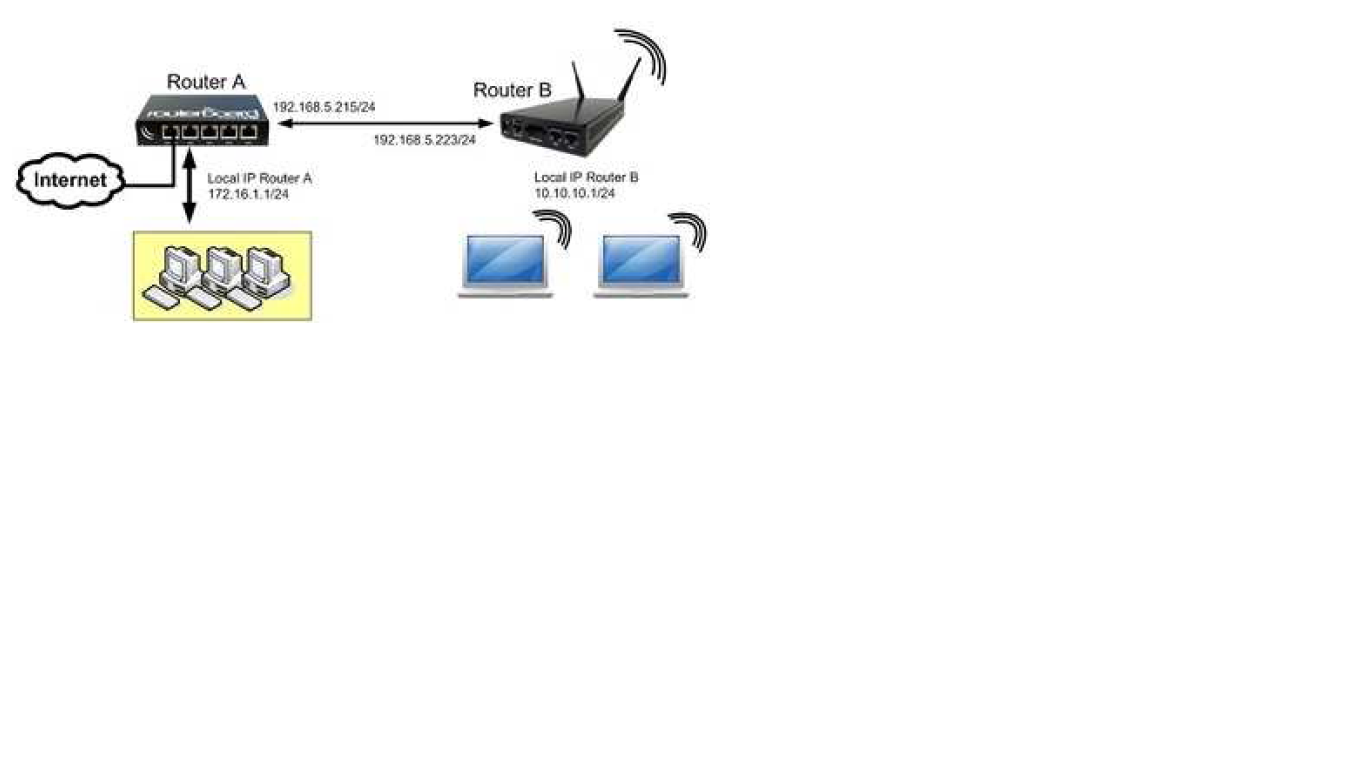
\includegraphics[width=13cm]{gambar/topologihotspot}
\caption{Gambar 2.2 Topologi HotSpot}
\end{figure}

%-------------------------------------------------------------------------------
\chapter{METODE PENELITIAN}
\section{Tempat dan Waktu Penelitian}
Penelitian proyek akhir ini dilaksanakan pada bulan Juni 2013 sampai dengan Agustus 2013 yang bertempat di Universitas Abulyatama Aceh Besar.

\begin{center}
Tabel 3.1. Jadwal Penelitian.
\end{center}
\vspace{-0.5cm}
\begin{figure}[ht!]
  \centering
    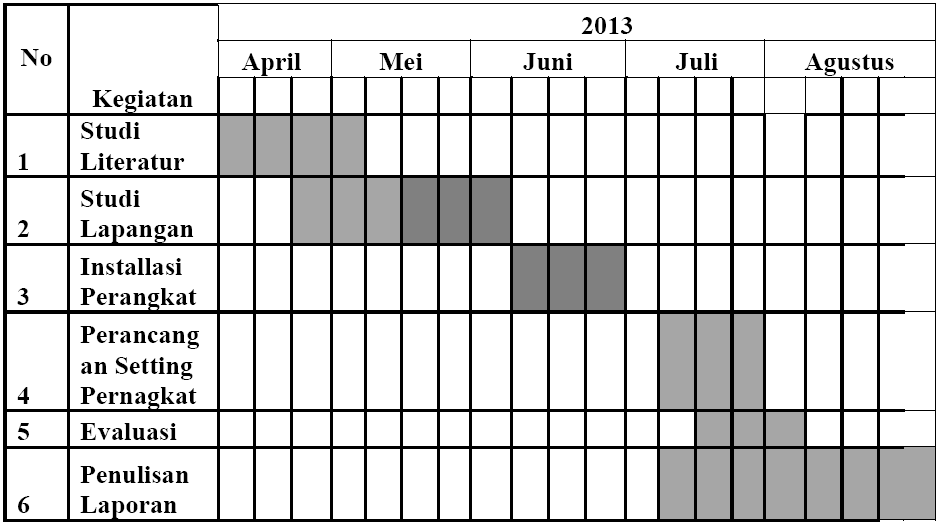
\includegraphics[width=13cm]{gambar/tabelkegiatan}
\end{figure}

\section{Alat dan Bahan}
Alat dan bahan yang digunakan dalam proses perancangan dan pembuatan HotSpot Server adalah sebagai berikut:

\vspace{-0.5cm}

\begin{enumerate}[a.]
\begin{singlespace}
\itemsep0em
\item Satu Unit PC/Laptop

Latop berfungsi untuk proses konfigurasi jaringan
\item  \emph{Router Board MikroTik} RB450G /  \emph{MikroTik RouterOS Level 4}

Router Board ini berfungsi sebagai server hotspot dan untuk manajemen jaringan,dengan level standart yaitu OS Level 4. Dalam perancangan ini tidak dibutuhkan fitur yang banyak, oleh karena itu tidak dibutuhkan level tinggi untuk rancangan ini dan juga dengan harga yang terjangkau.
\item \emph{Access Point}

AP berfungsi sebagai media jaringan hotspot. Perangkat yang digunakan adalah Ubiquiti NanoStation M2 dengan power yang cukup besar dan berkualitas tinggi.
\item  Kabel UTP Cat6 AMP

Kabel UTP Cat6e digunakan untuk penghubung jaringan dan juga power untuk koneksi AP ke POE dan Router. Dengan merk AMP original agar penggunaan bisa dalam jangka waktu yg lama dan untuk mengurangi masalah pada koneksi kabel. 
\item \emph{Winbox}

Winbox merupakan aplikasi remote yang di keluarkan mikrotik sendiri, berfungsi untuk mempermudah konfigurasi router dengan tampilan windows.
\item  \emph{Mozilla Firefox}

Mozilla berfungsi untuk percobaan browsing pada saat request access internet hingga muncul halaman login.
\end{singlespace}
\end{enumerate}

\section{Prosedur Kerja}
Untuk mendapatkan data dan informasi yang baik dan tepat, maka penulis menggunakan teknik sebagai berikut:

\vspace{-0.5cm}

\begin{enumerate}[1)]
\begin{singlespace}
\itemsep0em
\item Studi Literatur

Studi literatur adalah penelitian yang dilakukan untuk mendapatkan bahan rujukan berupa referensi yang bersifat teoristis dari buku-buku dan sumber bacaan lain yang dapat mendukung topik.

\item Persiapan \emph{software}

Tahapan ini dilakukan persiapan \emph{softeware} yang mendukung dalam perancangan sistem jaringan.

\item Pengambilan data lapangan

Data lapangan dibutuhkan sebagai data untuk perancangan jaringan \emph{Hotspot} dan dibutuhkan data mahasiswa untuk pembentukan \emph{User Manager} berupa NIM.

\item Perancangan Jaringan

Seluruh informasi dan survey lapangan akan dirancang membangun jaringan HotSpot

\item Analisa Hasil Simulasi

Tahapan ini merupakan tahapan analisa dari hasil uji coba serta melakukan perbaikan terhadap rancangan apabila ditemukan kekurangan atau kesalahan.
\end{singlespace}
\end{enumerate}



%-------------------------------------------------------------------------------
\chapter{HASIL DAN PEMBAHASAN}
\section{Perancangan Jaringan}
Berdasarkan hasil survei, pengamatan dan penerapan letak Access Point pada Gedung Kuliah Universitas Abulyatama, maka dapat di rencanakan sebuah jaringan HotSpot. Dalam perencanaan ini, tahap - tahapan yang harus dilakukan adalah sebagai berikut : 

Hasil Rancangan Penempatan AP (Access Point) dan Topologi Jaringan dapat dilihat pada Gambar 4.1 :

\vspace{-0.5cm}
\begin{figure}[ht!]
  \centering
    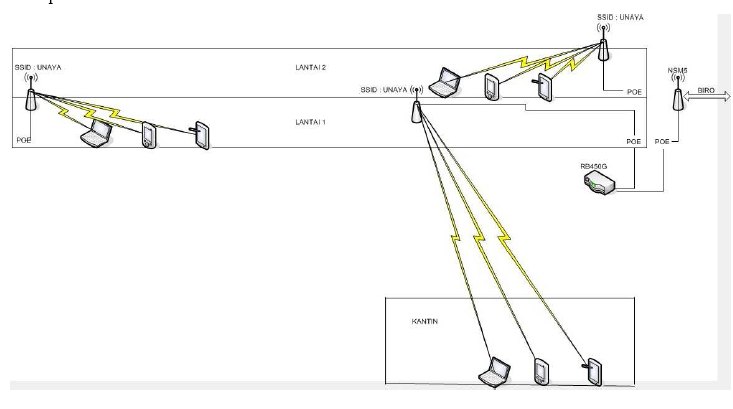
\includegraphics[width=13cm]{gambar/topologigedung}
\caption{Gambar 4.1 Topologi Jaringan Gedung Kuliah}
\end{figure}

Gedung kuliah memiliki 3(tiga) AP untuk HotSpot, dengan jarak AP Client ke AP utama Lebih-kurang 50-70 meter, dan panjang gedung  Lebih-kurang 100 meter. AP terpasang pada ujung gedung setiap lantai dengan posisi zigzag, agar setiap lantai 1 dan 2 bisa tercover sinyal dan juga tidak perlu memasang 2 AP setiap lantai. Gedung kuliah mengambil koneksi internet dari gedung BIRO dengan menggunakan wireless untuk koneksi point-to-point. Untuk koneksi ini menggunakan AP radio dengan frekwensi 5.8 GHz agar mengurangi serangan dari pihak yang tidak bertanggung jawab, karena device wireless pada perangkat yang biasa digunakan berbeda, yaitu 2.4 GHz, Seperti notebook, mobile phone, PDA dan lain sebagainya. Topologinya dapat dilihat pada Gambar 4.2

\vspace{-0.5cm}
\begin{figure}[ht!]
  \centering
    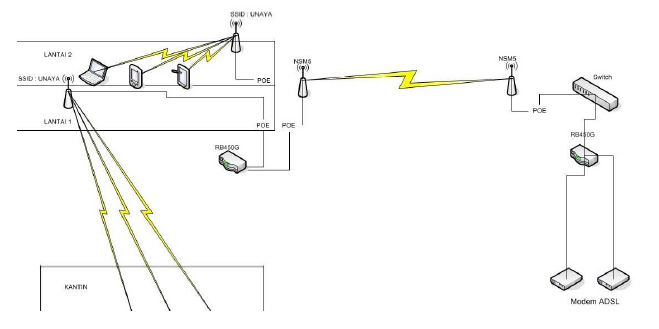
\includegraphics[width=13cm]{gambar/topologi2gedung}
\caption{Gambar 4.2 Topologi Jaringan antar gedung}
\end{figure}

Pada jaringan ini menggunakan topologi star untuk jaringan kabel dan WDS untuk topologi jaringan nirkabel.

\section{Perancangan Jaringan}
Tahap konfigurasi menggunakan aplikasi remote yaitu winbox. Aplikasi ini disediakan oleh mikrotik untuk memudahkan proses konfigurasi. Berikut adalah tahapan konfigurasi :
\subsection{Winbox}
Pada saat membuka apklikasi winbox pertama, yang berupa alamat perangkat, login, dan password.

\subsection{Penamaan Interface dan Penerapan IP Address}
Setiap interface yang digunakan di tandai dengan nama dan IP Address. Interface koneksi internet yang masuk di tandai dengan nama LAN-A yang mengambil koneksi internet dari gedung biro dengan IP Address 10.10.10.158/24. Penerapan IP Address mengikuti yang sudah di konfigurasi lebih dahulu oleh pihak Gedung A. Pada interface yang digunakan untuk HotSpot di berinama "AP" yang terkoneksi ke Access Point utama dengan IP Address 192.168.110.1/23 dengan network 192.168.110.0 dan broadcast 192.168.111.255 dengan artian range Address pool 192.168.110.2 - 192.168.111.254.

\subsection{Pembuatan Server hotspot}
Setelah penamaan interface dan penerapan IP Address, dilanjutkan pembuatan Server HotSpot. Pada step ini memilih interface "AP" sebagai interface yang akan digunakan untuk akses HotSpot. 

\begin{enumerate}[1)]
\begin{singlespace}
\itemsep0em
\item HotSpot address akan memilih network yang sudah di setting sebelumnya, yaitu 192.168.110.1/23 dan membuat Masquerade Network secara otoatis, ini untuk mengizinkan network tersebut bisa mengakses internet. 
\item Range IP pool yang diberikan oleh DHCP server pada client adalah dari 192.168.110.10 - 192.168.111.254, sedangkan IP range 192.168.110.2 - 192.168.110.9 untuk perangkat wireless.
\item Penentuan DNS yang ditujukan pada Gambar 4.8 merupakan DNS yang diberikan oleh pihak ISP, yaitu 125.160.10.2 sebagai Primary DNS dan 202.134.0.155 sabagai Secodary DNS.
\item Setelah selesai pembuatan HotSpot server, ada beberapa fitur yang dirubah, yaitu mengaktifkan fitur "Trial" pada "Server Profile" dan memberi durasi percobaan hanya satu jam.
\item Setelah satu jam login, koneksi internet secara otomatis akan terputus dan user tidak bisa menggunakan fitur trial lagi sebelum 24 jam, atau user bisa mengirim pesan singkat ke operator untuk membuat user hotspot berupa NIM.
\end{singlespace}
\end{enumerate}

\section{Configurasi Access Point}
\begin{enumerate}[1)]
\begin{singlespace}
\itemsep0em
\item Konfigurasi AP tidak memerlukan pengaman untuk mengakses jaringan wireless, hanya saja mengganti password konfigurasi AP dan beberapa konfingurasi yang harus di setting. 
\item Pada menu wireless hanya dirubah Wireless Mode ke "Access Point WDS" dan memberi SSID dengan nama "SEKOLAH" dan mengaktifkan mode auto dalam penerapan "WDS Peers" sebagai repeater atau AP Client.
\item Untuk memudahkan perubahan konfigurasi, setiap AP harus diberikan IP Address, masing - masing AP di beri IP 192.168.110.2, 192.168.110.3, dan 192.168.110.4. Pada menu ini, hanya AP Utama yang di aktifkan fitur "Spanning Tree Protocol" dan " Auto IP Aliasing".
\end{singlespace}
\end{enumerate}








%-----------------------------------------------------------------
%Disini akhir masukan Bab
%-----------------------------------------------------------------

%-----------------------------------------------------------------
%Disini awal masukan untuk Daftar Pustaka
%-----------------------------------------------------------------
%%\nocite{Abel2010,Guerbas201350}
%%\bibliography{research-plan}
%%\bibliographystyle{plainnat}
\begin{thebibliography}{9}

\bibitem[satu(2013)]{satu01}
http://id.wikipedia.org/wiki/MikroTik. Tanggal akses 6 Juni 2013.

\bibitem[dua(2013)]{dua02}
http://mikrotik.co.id/ Tanggal akses 6 Juni 2013.



\end{thebibliography}
\addcontentsline{toc}{chapter}{DAFTAR PUSTAKA}
%-----------------------------------------------------------------
%Disini akhir masukan Daftar Pustaka
%-----------------------------------------------------------------

\end{document}